\documentclass[conference]{IEEEtran}
\IEEEoverridecommandlockouts
% The preceding line is only needed to identify funding in the first footnote. If that is unneeded, please comment it out.
\usepackage{cite}
\usepackage{comment}
\usepackage{amsmath,amssymb,amsfonts}
\usepackage{algorithmic}
\usepackage{graphicx}
\usepackage{textcomp}
\usepackage{xcolor}
\usepackage{array}  % for better column formatting
\usepackage{color}  % to handle text color
\usepackage{algorithm}
\usepackage{algpseudocode}
\usepackage{amsmath}
\usepackage{float}
\usepackage{enumitem} % Enhanced list capabilities
\usepackage{hyperref}
\hypersetup{
    colorlinks=true,   % Ensures links can be clicked
    linkcolor=black,   % Makes links black, appearing as normal text
    citecolor=black,   % Ensures citation links are black
    pdfborder={0 0 0}, % Ensures there are no borders around links
    filecolor=black,   % Color for file links
    urlcolor=black     % Color for URL links, make black to appear as text
}
\usepackage{booktabs}


\def\BibTeX{{\rm B\kern-.05em{\sc i\kern-.025em b}\kern-.08em
    T\kern-.1667em\lower.7ex\hbox{E}\kern-.125emX}}
\begin{document}
\title{Hierarchical Clustering}
\author{\IEEEauthorblockN{Subir Balo}
\IEEEauthorblockA{\textit{Electronic Engineering} \\
\textit{Hamm-Lippstadt University of Applied Sciences}\\
Lippstadt, Germany \\
subir.balo@stud.hshl.de}
}
\maketitle

\begin{abstract}
This paper is focused on the exploration of the hierarchical clustering which is an effective method of gathering similar objects in the set. In Customer Segmentation, image recognition and gene analysis Hierarchical Clustering comes handy by exposing latent models. This research utilizes agglomerative methods which uses Euclidean and Manhattan distances to present clusters without determining their number in advance. Although it is computationally intensive and affected by extreme values, the hierarchical clustering provides a clear picture of the structure of data and becomes one of the most significant tools and methods in the data science.
\end{abstract}

\begin{IEEEkeywords}
Machine learning, ierarchical clustering, agglomerative, divisive, and Scikit-learn.
\end{IEEEkeywords}

\section{Introduction}
Hierarchical clustering is one of the basic algorithms employed in the machine learning for grouping of data into clusters. Another advantage that hierarchical clustering does not entail the actual number of groups to be determined or indicated in advance. However, it constructs a tree of clusters that can be visualized in the type of a tree called a dendrogram. Despite some drawbacks, this methodology is really helpful when working with large datasets and requiring to discover the data structure indeed.

There are two main types of hierarchical clustering, namely, agglomerative or bottom-up and divisive or top-down. However, the research topic of this paper is the agglomerative approach. It begins with each data point being a cluster and successively joins the two nearest clusters until there is only a single cluster left. This process produces a multi-level hierarchy of clusters that allows analysts to engage with data at multiple levels.\cite{nielsen2016introduction}

This particular kind of hierarchical clustering is commonly applied across the fields of image segmentation, social network analysis and in bioinformatics. In this paper, the various levels of agglomerative clustering and the various evaluation metrics that can be used to measure their effectiveness will be presented, and the strengths and weaknesses of the various levels discussed. Besides, the current paper will present an actual application of this methodology to solve a data segmentation issue.\cite{roux2018comparative}

The reader will have gained adequate exposure to the concept of hierarchical cluster, especially the agglomerative approach; and how the approach can be used in practical classification tasks.



\section{Types of Hierarchical Clustering}
Hierarchical clustering can be broadly categorized into two types: two major categories of clustering algorithms: the agglomerative (bottom-up) and divisive (top-down). Their methods and uses differ and this provides us with an advantage, depending on the kind of data analysis required to be done. the two methods of hierarchical clustering can be seen in the figure 1.\cite{day1984efficient}
\begin{figure}
    \centering
    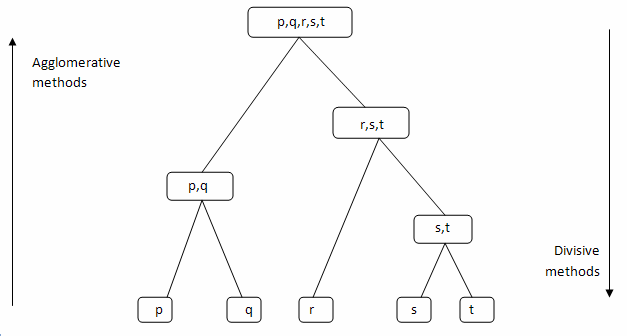
\includegraphics[width=0.9\linewidth]{Difference-between-agglomerative-and-divisive-hierarchical-clustering-methods.png}
\caption{(Hierarchical Clustering Agglomerative Vs Divisive - Google Search, n.d.\cite{Agglomerative_Vs_Divisive})}
    \label{fig:enter-label}
\end{figure}

\subsection{Agglomerative (Bottom-Up) Clustering}

There are two basic forms of clustering; of which the most widely used is the agglomerative clustering. The process starts with each data point as its own individual cluster, therefore the following steps are taken. Subsequently, it combines the two clusters of data that are nearest to one another based on the measure of dissimilarity before joining the other nearby clusters until the entire data set is bundled in a single cluster. This method can be visualized through the dendrogram noted on the Figure 2 below where the x-axis shows the data points and the y axis shows the distance of the cluster.\cite{nielsen2016introduction} The steps involved in agglomerative clustering are:

\begin{figure}
    \centering
    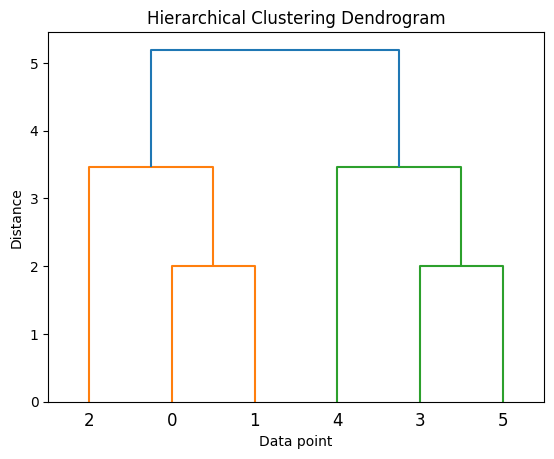
\includegraphics[width=0.7\linewidth]{Dendrogram.png}
    \caption{Dendrogram\cite{Dendrogram}}
    \label{fig:enter-label}
\end{figure}

\textbf{Calculate the Distance Matrix: }The next step which is calculating the pairwise distance between all data points should be performed.

\textbf{Find the Closest Clusters:} Find out which of the pair of clusters is closer to each other.

\textbf{Merge the Closest Clusters:} To do that we need to put these cluster in to one big cluster.

\textbf{Update the Distance Matrix:} Distance between the new cluster to all the remaining clusters must now be recalculated.

\textbf{Repeat:} Carry on with the merging and updating process until the final cluster which in this case is one is arrived at.

\subsection{Divisive (Top-Down) Clustering}
However, the presented dividing clustering is considerably different from the stated approach because it implies the more centralized perspective. K- means cluster begins with all instances assigned to the same cluster and iteratively breaks those line up into smaller and smaller line. It continues when all the points are grouped with their prototypes in separate clusters or when another condition is achieved. However, there are definitely some benefits one must consider when applying the divisive clustering, and those are quite notable especially in the case when the amount of data is initially small, and the further division occurs according to the data’s hierarchy. The steps in divisive clustering are:

\textbf{Start with All Data Points in One Cluster: }In this case, the cluster is taken as the whole database of instances.

\textbf{Split the Cluster:}By using the method for example the k-means clustering algorithm, one decomposes the given cluster into two miniature cluster.

\textbf{Repeat:}Go to split the least homogeneous group of data further and again continue the process until all the points get separated or until they do not reach another condition.

 \subsection{Types of Agglomerative Clustering
}Namely, agglomerative clustering is one of the approaches to division based on hierarchical clustering and a bottom-up approach. It moves forward beginning with each data point as one cluster and then links two at a time, the two closest clusters. The distribution of the distance between one cluster and the other obviously affects the clusters that are formed as a result. Distances between objects may be computed by several possibilities that are methods used to find this distance, referred to as linkage criteria. On the basis of agglomerative hierarchy the major forms include single linkage or nearest neighbor, complete linkage, average linkage as well as Ward's method.\cite{xu2005survey}\cite{roux2018comparative}

\textbf{Single Linkage Clustering:} Single linkage clustering measures the distance between two clusters as the minimum distance between any single pair of points, one from each cluster.It give the minimum distance between two points i and j based on the condition that i is a point of the cluster R and j is a point of cluster S.
\begin{equation}
L(R,S) = \min \{ D(i,j) \mid i \in R, j \in S \}
\end{equation}
\begin{figure}
    \centering
    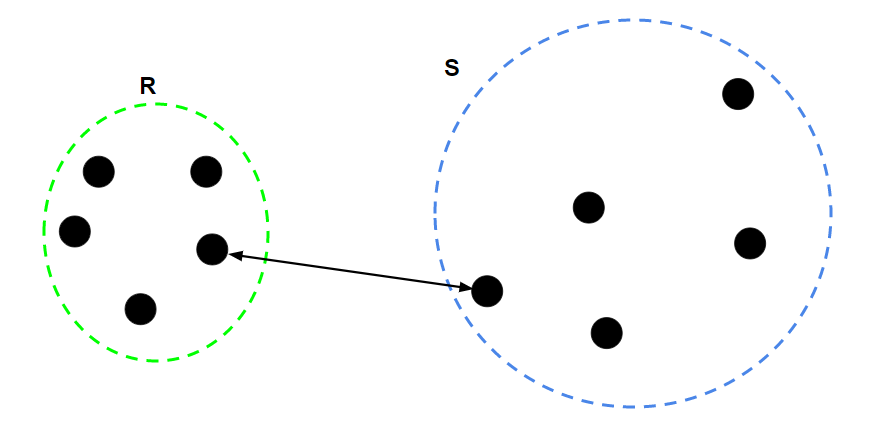
\includegraphics[width=0.6\linewidth]{single2.png}
    \caption{Single Linkage clustering\cite{Linkage}}
    \label{fig:enter-label}
\end{figure}

\textbf{Process:} Compute the distance matrix for all points.
Merge the two clusters with the smallest minimum distance between any pair of points. Update the distance matrix and repeat until all points are clustered.

\textbf{Advantages:} Simple to implement and computationally efficient.
Can handle non-elliptical shapes of clusters.

\textbf{Limitations:} Prone to the chaining effect, where clusters can form long, snake-like chains, linking together points that might not be close overall.

\textbf{Average Linkage Clustering:} Average linkage clustering , estimates the distance between two clusters for example, by taking the mean of the distance between each point in one cluster and each point in the other cluster.Similarly, for two clusters R and S, first for every data-point i of R and every data-point i of S, the distance between them is found out, and then the average of all these distances is calculated. Based on the assumption of Average Linkage, this is the value of the arithmetic mean.\cite{roux2018comparative}
\begin{equation}
L(R,S) = \frac{1}{n_R \times n_S} \sum_{i=1}^{n_R} \sum_{j=1}^{n_S} D(i,j), \quad i \in R, j \in S
\end{equation}
\begin{figure}
    \centering
    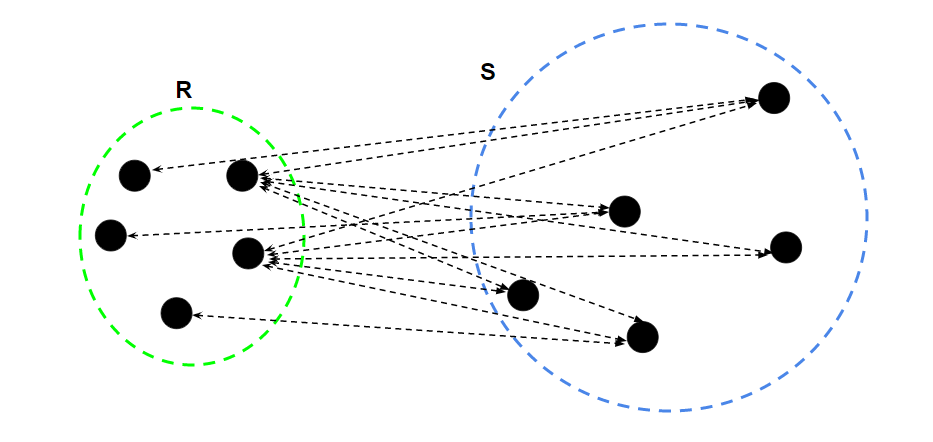
\includegraphics[width=0.6\linewidth]{average linkage.png}
    \caption{Average Linkage\cite{Linkage}}
    \label{fig:enter-label}
\end{figure}

\textbf{Process:} Calculate the distances of all the points, that is, find the distance matrix.
It is required to join the two clusters that have the least average of the distances of all the points with each other. Proceed by updating the distance matrix and continue this process for all the points to cluster.

\textbf{Advantages:} Solves the problems that are caused by both run and complete linkage. It is relatively less affected with regard to outliers compared to complete linkage.   

\textbf{Limitations:} Frequently more computationally expensive than single linkage. May not work well when you need the semblance of groups which are in very different shapes.

\textbf{Complete Linkage Clustering:}
Complete linkage clustering measures the distance between two clusters as the maximum distance between any single pair of points, one from each cluster.For two clusters R and S, the complete linkage gives the maximum of distance between any two points i and j, where i ∈ R and, j ∈ S.\cite{xu2005survey}

\begin{equation}
L(R,S) = \max \{ D(i,j) \mid i \in R, j \in S \}
\end{equation}

\begin{figure}[H]
\centering
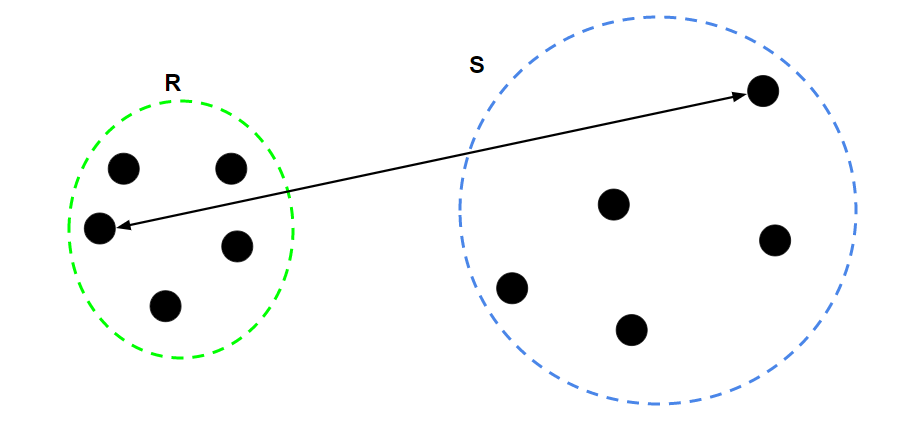
\includegraphics[width=.4\textwidth]{complete linkage.png}
\caption{Linkage\cite{Linkage}}
\label{DPE}
\end{figure}

\textbf{Process:}
Compute the distance matrix for all points.
Merge the two clusters with the smallest maximum distance between any pair of points.
Update the distance matrix and repeat until all points are clustered.Advantages:
Tends to create more compact clusters compared to single linkage.
Reduces the chaining effect.

\textbf{Limitations:}
More computationally intensive than single linkage.
Sensitive to outliers and noise.

\textbf{Ward’s Method:}
Ward’s method measures the distance between two clusters as the increase in the total within-cluster variance when they are merged.\cite{xu2005survey}

\begin{figure}
    \centering
    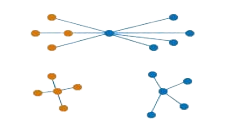
\includegraphics[width=0.6\linewidth]{ward_s_method-removebg-preview.png}
    \caption{Ward's method\cite{wardmethod}}
    \label{fig:enter-label}
\end{figure}

\textbf{Process:}
Compute the initial variance for all individual points.
Merge the two clusters that result in the smallest increase in total within-cluster variance.
Update the variance and repeat until all points are clustered.

\textbf{Advantages:}
Produces clusters with minimal variance, often leading to very compact and spherical clusters.
Reduces the impact of outliers compared to other methods.

\textbf{Limitations:}
Computationally expensive due to the need to calculate variances.
Assumes spherical clusters, which might not be suitable for all datasets.

\subsection{Determining the distance between two points}
Before carrying out clustering it is necessary to measure the degree of resemblance or non-likeness of the data. The two distances that are often used include Euclidean and Manhattan. Understanding the distances between the points within the space helps in determining the clusters and these metrics are of help in this aspect.\cite{xu2005survey}\cite{yim2015hierarchical}
\begin{figure}
    \centering
    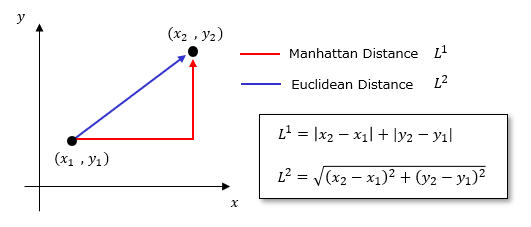
\includegraphics[width=0.8\linewidth]{Euclidean and Manhatten distance.png}
    \caption{The Euclidean and Manhatten Distance.\cite{TheEuclideanandManhattenDistance}}
    \label{fig:enter-label}
\end{figure}

\textbf{The  Euclidean distance:}The Euclidean distance between two points is the distance of these two points in a straight line when these points are located in n-dimensional space. This distance measure is the most popular one; actually it is a measure of distance in terms of lengths between the two points.\cite{yim2015hierarchical} This distance is shown as the blue line in the figure 7.

\textbf{The Manhatten distance:}The Manhattan distance better known as the L1 distance or the city block distance is a way of describing the distance between two points where the distance is the sum of the absolute differences between their coordinates. This metric is as if you have to move in a city map that has the roads interconnecting only at 90-degree angles.\cite{yim2015hierarchical} In the figure 7, this is presented as red colour along the grid lines in the graphic as depicting the distance of movement.

\subsection{Hierarchical Clustering for Segmentation of Customers} Customer segmentation is acknowledged as one of the most important activities in marketing and business information processing. It refers to the process of categorising customers depending with their attributes and actions to enhance market strategies and thus the satisfaction of customers. For this purpose, the method that could be used is agglomerative hierarchical clustering for it identifies the hierarchal characteristics in the dataset without providing the number of clusters in advance. This section further explains agglomerative clustering for customer segmentation and performs the same on a sample dataset and visualizes the result by a dendrogram.\cite{salvador2004determining}

\textbf{Dataset Overview:} The dataset used for customer segmentation includes the following attributes:

\textbf{CustomerID:} To avoid confusion of customers’ data, this field has characteristics of unique identification of each customer.

\textbf{Genre:} Male or female of the customer.

\textbf{Age: }The five disrupted areas are the age of the customer.

\textbf{Annual Income (k-USD)}: An annual income of the customer in thousand US dollars.

\textbf{Spending Score (1-100):} This is the actual spending score given by the store often in accordance to the user’s behavior or spending habits.

Here is a snippet of the dataset:
\begin{figure}
    \centering
    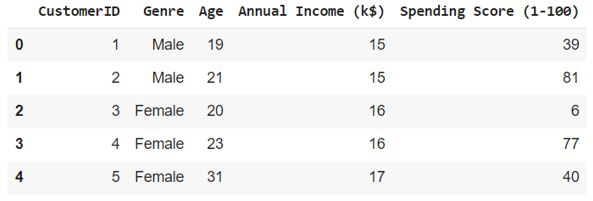
\includegraphics[width=0.8\linewidth]{customer segmentation.JPG}
    \caption{customer data}
    \label{fig:enter-label}
\end{figure}

\textbf{The following is a code for implementing agglomerative clustering:}
The figure 9 and 10 are the Python code. It explains how to carry out Agglomerative clustering on the given customer dataset using Ward linkage and show the output in the form of a dendrogram.

\noindent The whole code is available on GitHub in the following lin with the name 'Hierarchical clustering Implementation.ipynb' in the repository:
\href{https://github.com/hammadkaramat/Autonomous-lab-truck-platooning-/blob/main/Hierarchical%20clustering%20Implementation.ipynb}{\textbf{Visit GitHub}}


\begin{figure}
    \centering
    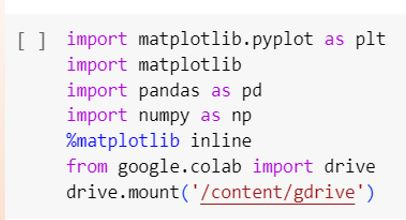
\includegraphics[width=0.7\linewidth]{code snip for customer segmentation.JPG}
    \caption{Code snippet }
    \label{fig:enter-label}
\end{figure}

\begin{figure}
    \centering
    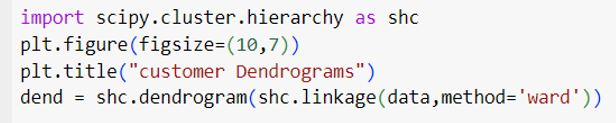
\includegraphics[width=0.6\linewidth]{result snip for customer segmentation.JPG}
    \caption{Code snippet}
    \label{fig:enter-label}
\end{figure}

\textbf{Interpretation of the Dendrogram}
This dendrogram as generated by the above code is a tree like structure aimed at depicting the hierarchical relationship of the data values. Each of the merge in the dendrogram characterize the amalgamation of two clusters which are simply similar to each other. This is the extent of the merge, where the vertical axis measures height, which can be the distance between the two clusters that are merging.

In the dendrogram:

Lower merges are formation of similar clusters with the clusters having closer means.
Higher merges mean merging of similar clusters Which means the clusters being merged are less similar to each other.
Horizontal lines are equal clusters and the vertical lines between them as indicating where they became integrated.
Results
This dendrogram presents the hierarchy of the customers’ groups according to the annual income and the spending level. The works also described that to decide the right number of clusters one must follow a line that is absolutely vertical and does not touch the horizontal lines (also known as cutting the dendrogram).

The dendrogram visualized in the result indicates distinct customer segments that can be targeted with specific marketing strategies.\cite{roux2018comparative}

\begin{figure}
    \centering
    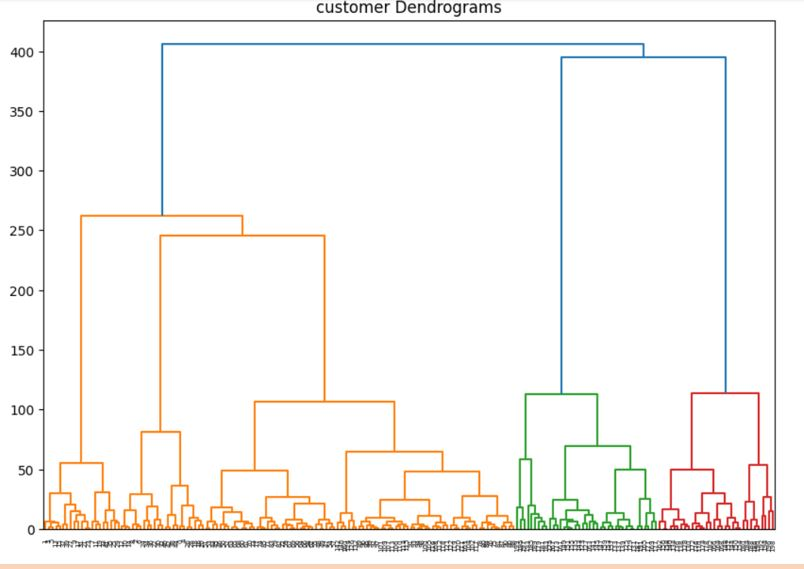
\includegraphics[width=0.6\linewidth]{Dendograms for customer segmentation.JPG}
    \caption{Dendograms for customer segmentation}
    \label{fig:enter-label}
\end{figure}

\section{Conclusion}
Overall, hierarchical clustering, especially the agglomerative one, is one of the most essential clustering techniques that proves to be effective for identifying the subtle structures within huge datasets. From this paper, an illustration of its application in customer segmentation was done using the program to show the details of how linkage criteria such as single, complete, average, and Ward’s method can group customers’ behaviors with similar characteristics and distances using links such as the Euclidean and Manhattan. In the practical application this helped to demonstrate how effectively the method could be used in establishing valuable customer segments with the help of dendrogram. Although, hierarchical clustering is beneficial in representing the guidelines of number of clusters which is not possible in other methods and providing detailed trees of the hierarchical structure, it also has certain disadvantages such as high computational time and problems with outliers. These form challenges call for upgrades in aspects such as algorithms that are least sensitive to noise and a better computational facility. In general, hierarchical clustering is a convenient and essential method in a wide variety of contexts and areas such as customer classification, image and gene analysis; therefore, it is critical for enhancing the work’s stability and flexibility for future studies.

\bibliographystyle{plain}
\bibliography{mybib}
\end{document}
